\documentclass{beamer}
\usepackage[utf8]{inputenc}

\usetheme{Madrid}
\usecolortheme{default}
\usepackage{amsmath,amssymb,amsfonts,amsthm}
\usepackage{txfonts}
\usepackage{tkz-euclide}
\usepackage{listings}
\usepackage{adjustbox}
\usepackage{array}
\usepackage{tabularx}
\usepackage{gvv}
\usepackage{lmodern}
\usepackage{gensymb}
\usepackage{circuitikz}
\usepackage{tikz}
\usepackage{graphicx}

\setbeamertemplate{page number in head/foot}[totalframenumber]

\usepackage{tcolorbox}
\tcbuselibrary{minted,breakable,xparse,skins}



\definecolor{bg}{gray}{0.95}
\DeclareTCBListing{mintedbox}{O{}m!O{}}{%
  breakable=true,
  listing engine=minted,
  listing only,
  minted language=#2,
  minted style=default,
  minted options={%
    linenos,
    gobble=0,
    breaklines=true,
    breakafter=,,
    fontsize=\small,
    numbersep=8pt,
    #1},
  boxsep=0pt,
  left skip=0pt,
  right skip=0pt,
  left=25pt,
  right=0pt,
  top=3pt,
  bottom=3pt,
  arc=5pt,
  leftrule=0pt,
  rightrule=0pt,
  bottomrule=2pt,
  toprule=2pt,
  colback=bg,
  colframe=orange!70,
  enhanced,
  overlay={%
    \begin{tcbclipinterior}
    \fill[orange!20!white] (frame.south west) rectangle ([xshift=20pt]frame.north west);
    \end{tcbclipinterior}},
  #3,
}
\lstset{
    language=C,
    basicstyle=\ttfamily\small,
    keywordstyle=\color{blue},
    stringstyle=\color{orange},
    commentstyle=\color{green!60!black},
    numbers=left,
    numberstyle=\tiny\color{gray},
    breaklines=true,
    showstringspaces=false,
}
%------------------------------------------------------------
%This block of code defines the information to appear in the
%Title page
\title %optional
{1.11.13}
%\subtitle{A short story}

\author % (optional)
{AI25BTECH11011-VARUN}


\begin{document}


\frame{\titlepage}
\begin{frame}{Question}

If a line makes angles 90$\degree$,135$\degree$,45$\degree$ with the x, y and z axes respectively,find its direction cosines.

\end{frame}

\begin{frame}{Theoretical Solution}

The direction cosines of a vector $\vec{A}$ making $\alpha$, $\beta$ and $\gamma$ angles with x,y and z axes respectively is,

\begin{align}
    \vec{A} = \myvec{\cos{\alpha} \\ \cos{\beta} \\ \cos{\gamma}}
\end{align}

Then, the direction vector is,

\begin{align}
    \vec{A} = \myvec{\cos{90\degree} \\ \cos{135\degree} \\ \cos{45\degree}}  \\
    \vec{A} = \myvec{0 \\ -\frac{1}{\sqrt{2}} \\ \frac{1}{\sqrt{2}}}
\end{align}

\end{frame}


\begin{frame}[fragile]
    \frametitle{main C Code}

    \begin{lstlisting}
#include <stdio.h>

void find_direction_cosines(int alpha_deg, int beta_deg, int gamma_deg, double *l, double *m, double *n);

int main(){
    double l, m, n;
    find_direction_cosines(90, 135, 45, &l, &m, &n);
    printf("Direction cosines:\nl = %.4lf\nm = %.4lf\nn = %.4lf\n", l, m, n);
    return 0;
}
    \end{lstlisting}
\end{frame}

\begin{frame}[fragile]
    \frametitle{C Code}
    
    \begin{lstlisting}
#include <math.h>

double degree(int n){
    double d = (n * M_PI) / 180;
    return d;
}

void find_direction_cosines(int alpha_deg, int beta_deg, int gamma_deg, double *l, double *m, double *n) {
    *l = cos(degree(alpha_deg));
    *m = cos(degree(beta_deg));
    *n = cos(degree(gamma_deg));
}
    \end{lstlisting}
\end{frame}

\begin{frame}[fragile]
    \frametitle{Python Code}
    \begin{lstlisting}
import ctypes
import numpy as np
import matplotlib.pyplot as plt

lib = ctypes.CDLL('./libdirection.so')
lib.find_direction_cosines.argtypes = [
    ctypes.c_int, ctypes.c_int, ctypes.c_int,
    ctypes.POINTER(ctypes.c_double), ctypes.POINTER(ctypes.c_double), ctypes.POINTER(ctypes.c_double)
]

l = ctypes.c_double()
m = ctypes.c_double()
n = ctypes.c_double()

lib.find_direction_cosines(90, 135, 45, ctypes.byref(l), ctypes.byref(m), ctypes.byref(n))
    \end{lstlisting}
\end{frame}

\begin{frame}[fragile]
    \frametitle{Python Code}
    \begin{lstlisting}
print(f"Direction cosines:\nl = {l.value}\nm = {m.value}\nn = {n.value}")

fig = plt.figure()
ax = fig.add_subplot(111, projection='3d')

origin = np.array([0, 0, 0])
vector = np.array([l.value, m.value, n.value])

ax.quiver(origin[0], origin[1], origin[2],
          vector[0], vector[1], vector[2],
          length=1, normalize=True, color='red')
ax.set_xlim([-1, 1])
ax.set_ylim([-1, 1])
ax.set_zlim([-1, 1])
ax.set_xlabel('X axis')
ax.set_ylabel('Y axis')
ax.set_zlabel('Z axis')
    \end{lstlisting}
\end{frame}

\begin{frame}[fragile]
    \frametitle{Python Code}
    \begin{lstlisting}
ax.set_title('Direction Cosines Vector')
plt.savefig("/home/gara-varun-kumar/ee1030-2025/ai25btech11011/matgeo/1.11.13/figs/Fig 1.png")
plt.show()
    \end{lstlisting}
\end{frame}

\begin{frame}{Plot}
    \centering
    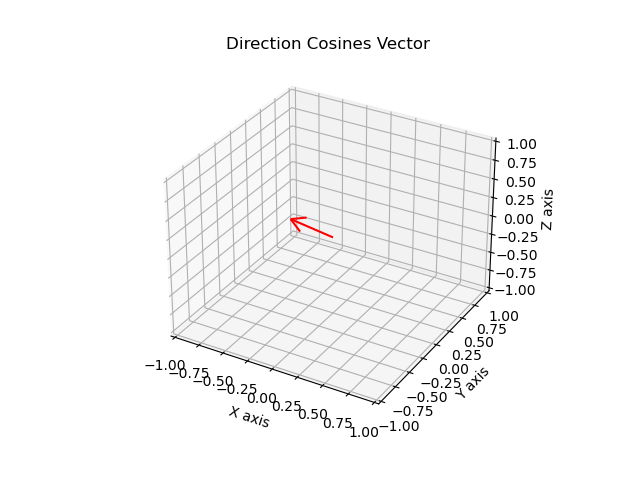
\includegraphics[width=\columnwidth, height=0.8\textheight, keepaspectratio]{figs/Fig 1.png}     
\end{frame}

\end{document}
